%preamble
\documentclass[letterpaper]{article}
\synctex=1
\usepackage{graphicx}
\graphicspath{ {images/} }

\usepackage{lipsum}
\usepackage{float}
% \bibliographystyle{IEEEtran}
% \bibliographystyle{ieeetr}

\usepackage{amssymb}

\usepackage{siunitx}

\usepackage{multirow}
% for merging table cells I think

\usepackage{fancyhdr} %header
\fancyhf{}
\fancyhead[R]{Arun Woosaree XXXXXXX}
\renewcommand\headrulewidth{0pt}
\fancyfoot[C]{\thepage}
\renewcommand\footrulewidth{0pt}
\pagestyle{fancy}

% make subsection use letters
\renewcommand{\thesubsection}{\thesection.\alph{subsection}}

%actual document
\begin{document}

% \maketitle %insert titlepage here
\begin{titlepage}
 \begin{center}
  \vspace*{1cm}
  \Huge
  Stat 235
  \vspace{1cm}
  
  Lab 3
  \vspace{1cm}
  
  WOOSAREE, Arun
  \vspace{1cm}
  
  \Huge
  Lab EL12
  \vspace{1cm}
  
  TA: Jessa Marley
  \vspace{1cm}
  
  \today
  \vfill
 \end{center}
\end{titlepage}

\section{}%1
% Use Poisson probabilities sheet.
% How does change in lambda affect shape of graph?
% How does the increase affect the quality/number of flaws?
As $\lambda$ increases, the distribution shifts to the right, since $\lambda$ is
the mean value of the distribution. We also see that as this distibution shifts
to the right, the curve flattens as a result of the mean probability decreasing
while the spread increases. Since Poisson distributions measure the number of
successes in an interval, and in this case a ``success'' is a flaw in a plastic
panel, we can clearly see that as $\lambda$ increases, the number of flaws in
the plastic panels also increase.

\section{}%2

\subsection{}%2a
% Use Poisson probabilities sheet
% What value should x have?
Assuming $\lambda=0.5$, the probability that there are no flaws in a randomly
selected panel is $P(X=0)$. Using the \textit{Poisson Probabilities} worksheet,
we find this number to be $0.6065$, or $60.65\%$ of the panels are in perfect
condition

\subsection{}%2b
% Use Poisson probabilities sheet
% What probability should go in the distribution? Choose carefully

\subsection{}%2c
% Use Poisson probabilities sheet
% MAYBE there's something useful in part b .. think of them as 10 independent events
% ex: how do we find trhe probability of getting 2 heads in a row for a coin toss?
% 1/2 * 1/2 = 1/4

\section{}%3

\subsection{}%3a
% Use the normal probabilities sheet
% Why can't we assume that the distribution of the sample mean is normal?
% (Think sample size, central limit theorem)
% Find the variance and mean to get probability

\subsection{}%3b
% Use the normal probabilities sheet
% Why can't we assume that the distribution of the sample mean is normal?
% (Think sample size, central limit theorem)
% Find the variance and mean to get probability

\section{}%4
% DO NOT CHANGE THE FORMULAS IN THE ROWS AVERAGE, COUNT, AVERAGE summary statistics

\subsection{}%4a
% Use Simulation sheet in cells B9:BI18
% Random number generation -> #variables=60 -> randomvars=10
% -> distribution=Poisson -> seed=100 -> lambda=COUNTIF()

\subsection{}%4b
% count will be in row 42 if you generated the data correctly

\subsection{}%4c
% Don't over analyze, use squint test
% What's going on between 0.3 and 0.7?

\begin{figure}[H]
 \centering
 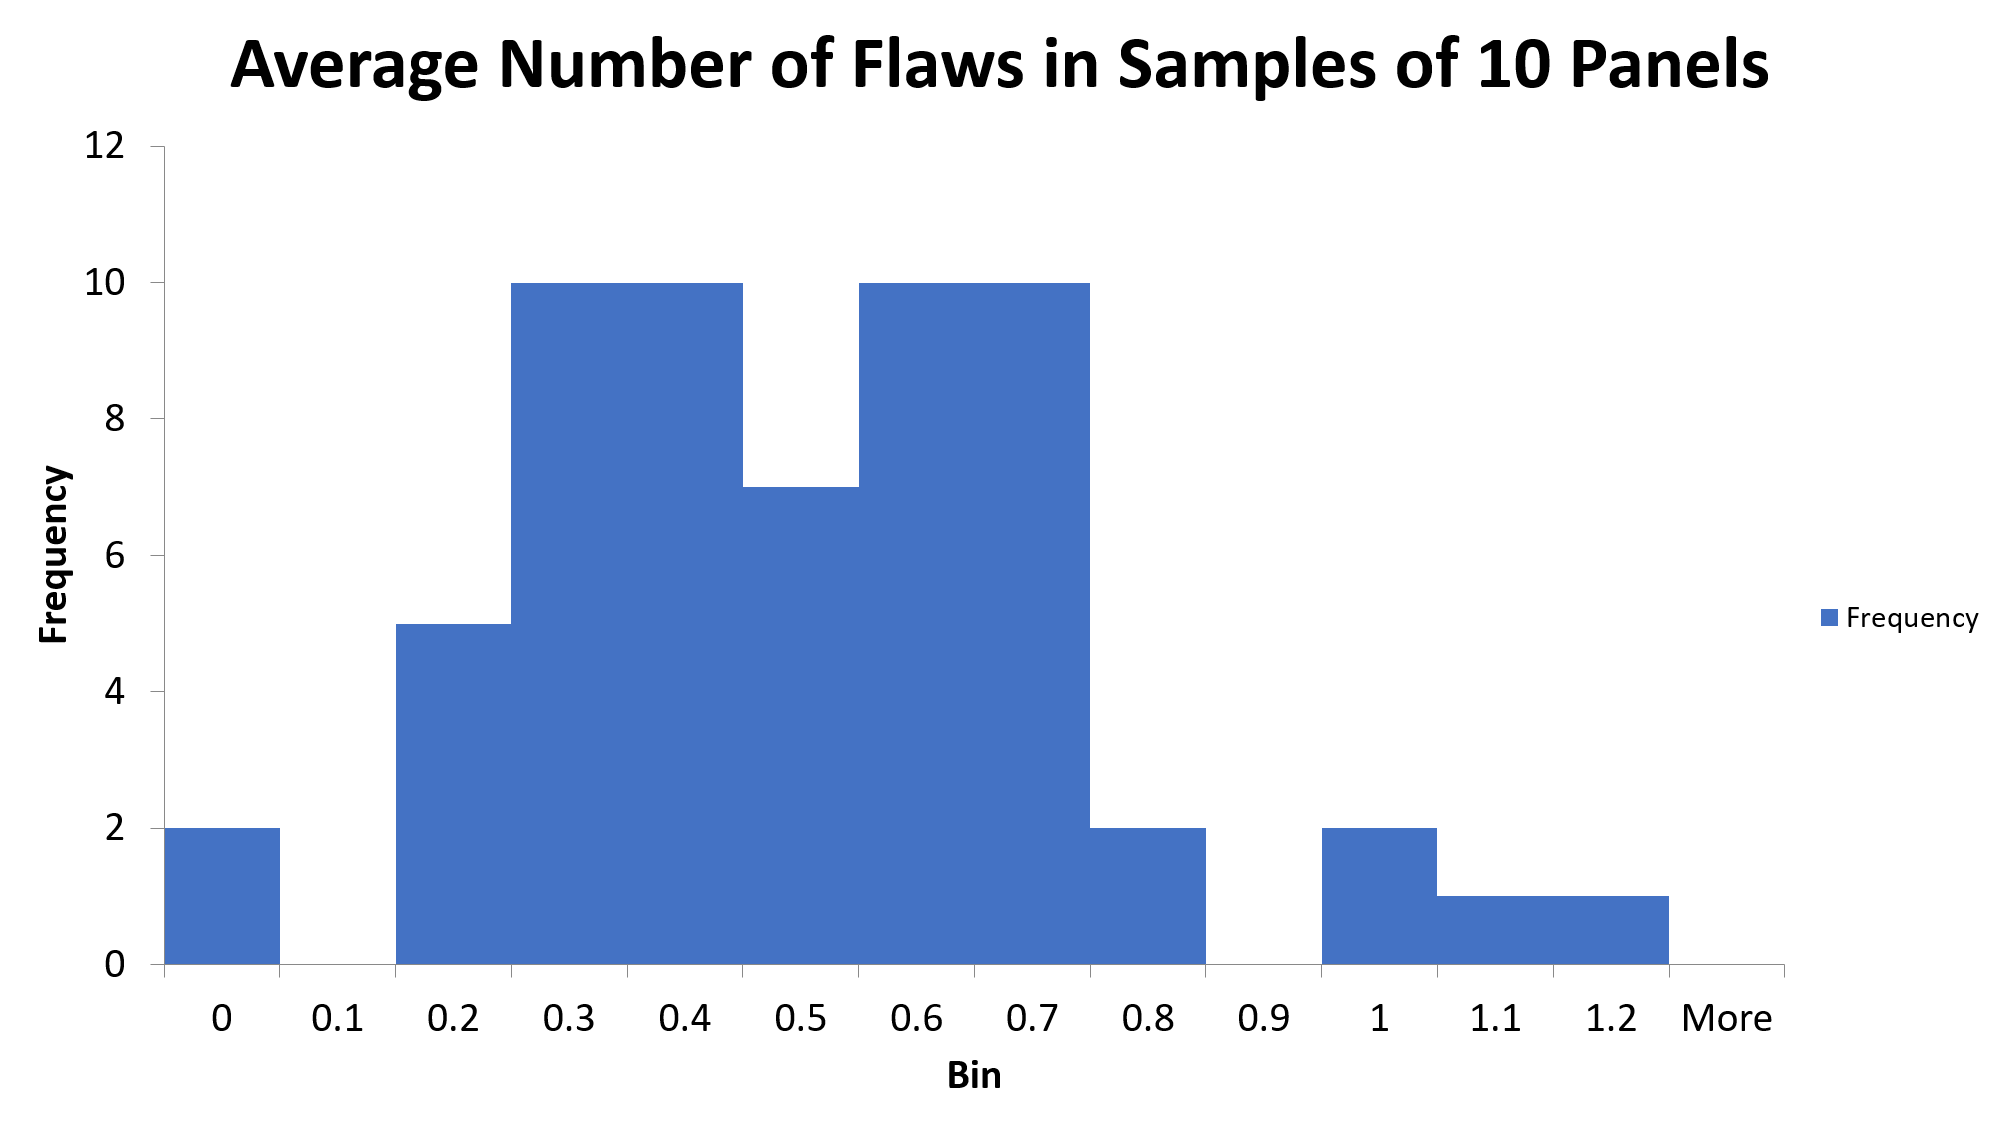
\includegraphics[width=\textwidth]{q4.png}
 \caption{INSERT CAPTION HERE}
 \label{4c}
\end{figure}

\subsection{}%4d
% Summary statistics calculated automatically.
% Are the predicted values close?
% If they aren't perfect, why not?

\section{}%5

\subsection{}%5a
% Basically, repeat question 4c, d with n=30
% Redo the random simulation
% When comparing, how does the central limit theorem apply?

\begin{figure}[H]
 \centering
 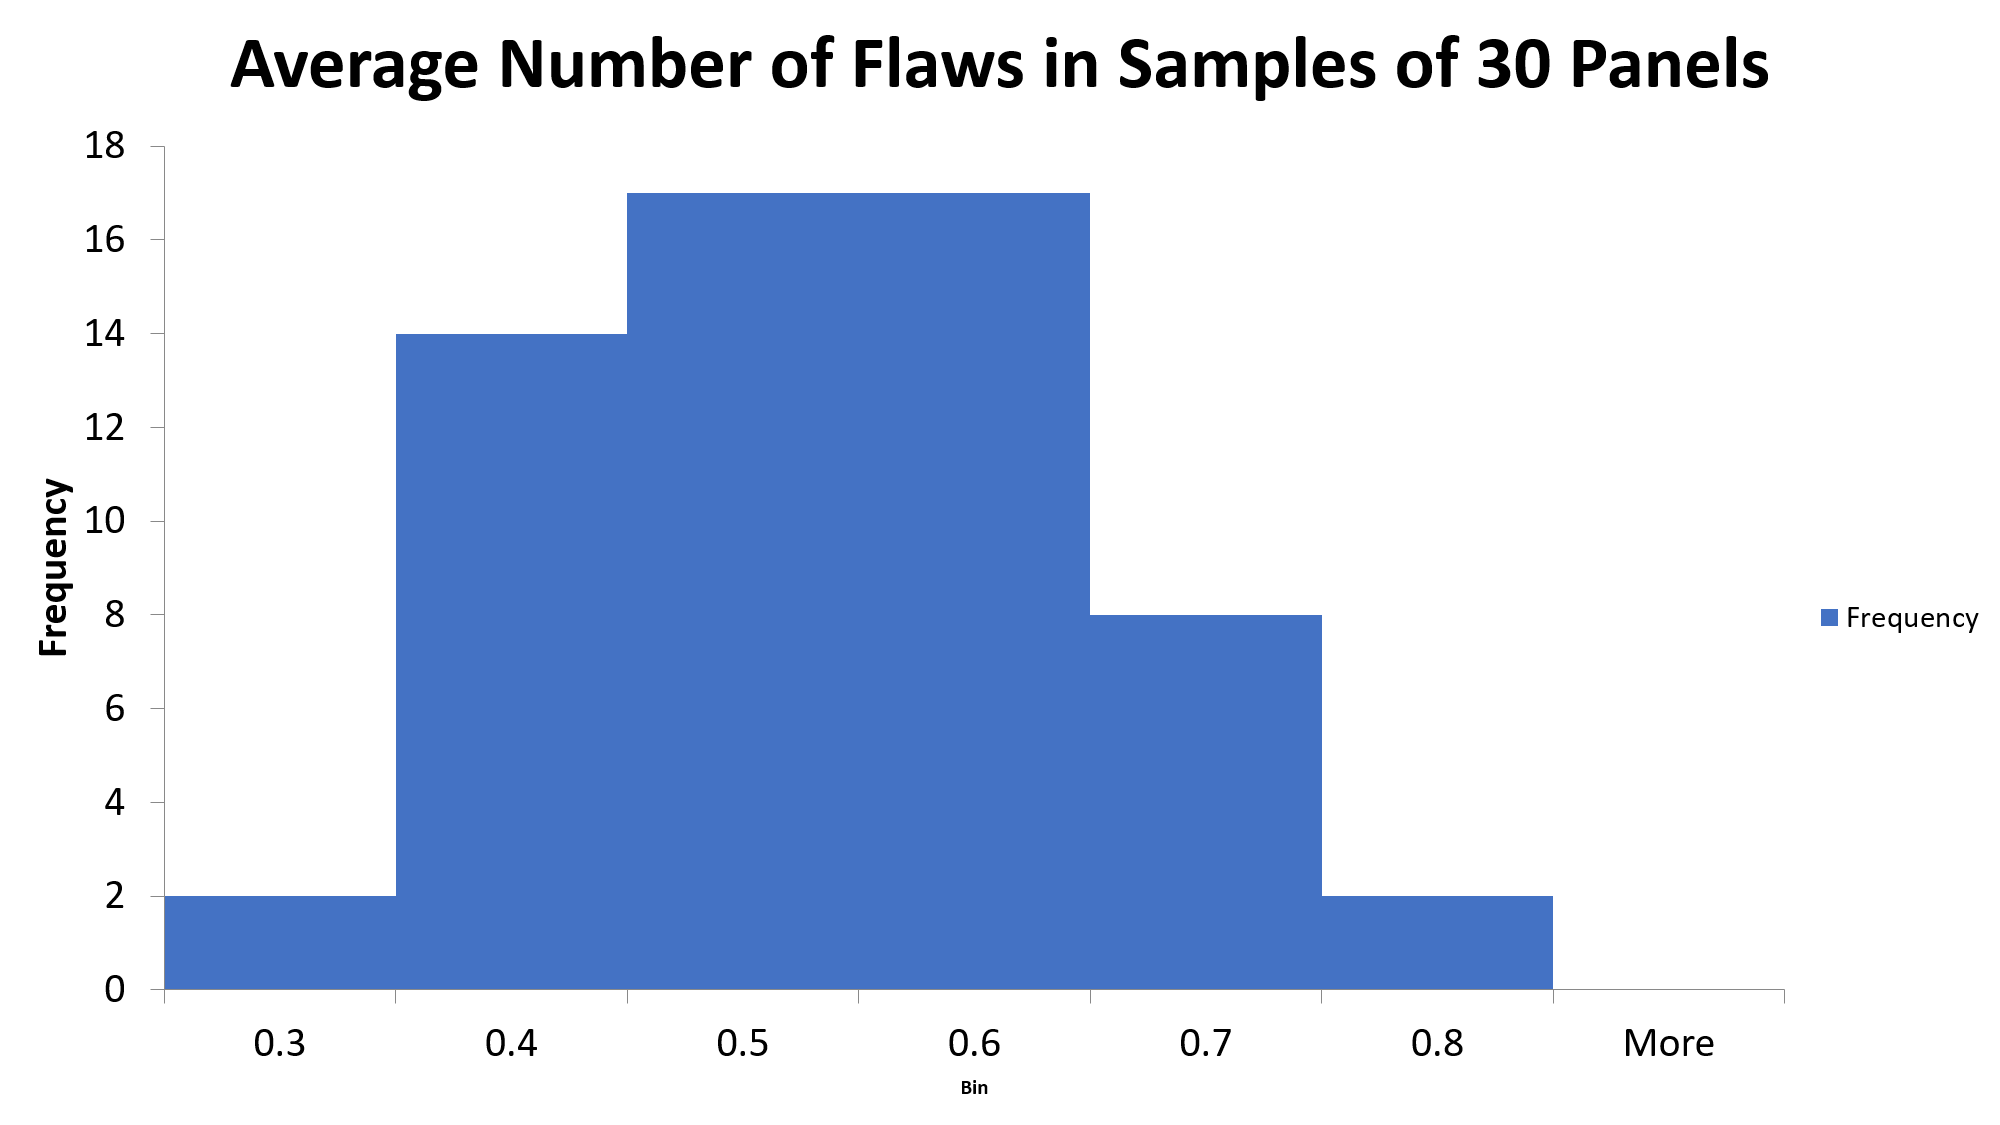
\includegraphics[width=\textwidth]{q5.png}
 \caption{INSERT CAPTION HERE}
 \label{5a}
\end{figure}

\subsection{}%5b
% Why is this estimate better/worse?


\end{document}
